\documentclass{beamer}

% ===============================
% Theme and Packages
% ===============================
\usetheme{Madrid}
\usecolortheme{default}
\usefonttheme{professionalfonts}

\usepackage{amsmath, amssymb}
\usepackage{graphicx}
\usepackage{booktabs}
\usepackage{hyperref}
\usepackage{setspace}
\usepackage{ragged2e} 
\usepackage{setspace} 

% ===============================
% Title Information
% ===============================
\title[Towards Automated Circuit Discovery]{Towards Automated Circuit Discovery\\for Mechanistic Interpretability}
\date{}

% ===============================
% Document
% ===============================
\begin{document}
	
	%------------------------------------------------
	% Title Slide
	%------------------------------------------------
	\begin{frame}
		\centering
		{\Large\bfseries Towards Automated Circuit Discovery\\[4pt]
			for Mechanistic Interpretability}
		
		\vspace{20pt}
		
		{\small
			Arthur Conmy, Augustine N. Mavor-Parker, Aengus Lynch,\\
			Stefan Heimersheim, Adri\`a Garriga-Alonso}
		
		\vspace{8pt}
		
		\vfill
		
		{\small
			Presented by: \textbf{Anbuselvi S}}
	\end{frame}
	
	\begin{frame}{Presentation Outline}
		\begin{itemize}
			\setstretch{1.6}
			\item Motivation and Background
			\item Circuits and Scalability Challenges
			\item Common Workflow for Circuit Discovery
			\item Automatic Circuit Discovery (ACDC)
			\begin{itemize}
				\item behavior and dataset setup
				\item computational graph representation
				\item activation patching and recursive pruning
			\end{itemize}
			\item Evaluation Methodology
			\item Related Work
			\item Limitations
			\item Conclusion
		\end{itemize}
	\end{frame}
	
	%------------------------------------------------
	% 1 - Motivation and Mechanistic Interpretability
	%------------------------------------------------
	\begin{frame}{Motivation and Mechanistic Interpretability}
		\begin{itemize}
			\setstretch{1.4}
			\item Rapid progress in \textbf{transformer language models}
			has led to new and complex emergent capabilities.
			\item Despite strong predictors of performance, transformers
			remain widely viewed as \textbf{black-box models}.
			\item Interpretability research seeks to:
			\begin{itemize}
				\item demystify model behavior
				\item explain outputs using domain-relevant concepts
			\end{itemize}
			\item \textbf{Mechanistic interpretability} focuses on
			reverse-engineering model internals into
			\textbf{human-understandable algorithms}.
		\end{itemize}
	\end{frame}
		
	%------------------------------------------------
	\begin{frame}
		\vspace*{6pt}
		\textbf{Can the discovery of behavior-specific circuits inside neural networks
		be automated rather than relying on manual mechanistic analysis?}
		
		\vspace{26pt}
			\centering
		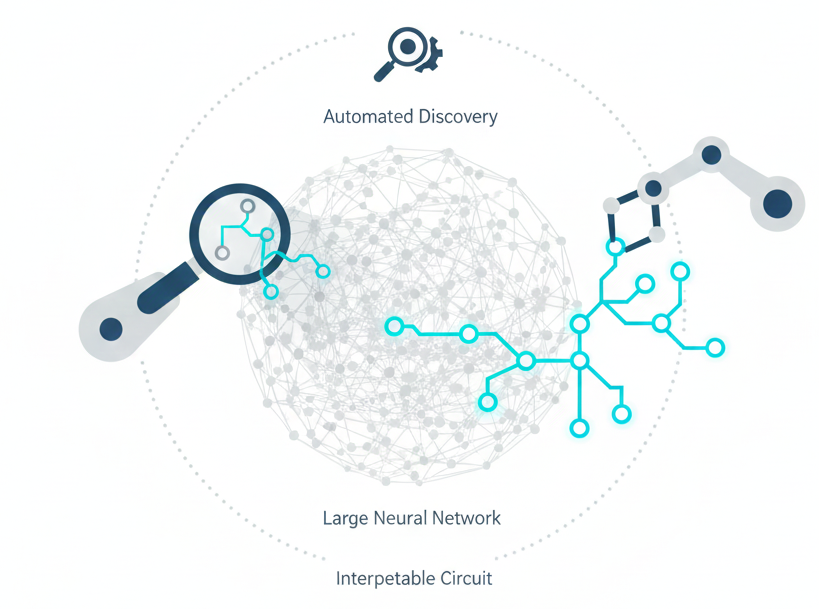
\includegraphics[width=0.6\textwidth]{fig.png}
	\end{frame}
	
	%------------------------------------------------
	% 2 - Circuits and the Scalability Problem
	%------------------------------------------------
	\begin{frame}{Circuits and the Scalability Problem}
		\begin{itemize}
			\setstretch{1.7}
			\item \justifying
			Model behaviors are implemented by algorithms within the model’s
			\textbf{computational graph}, and \textbf{circuits} correspond to
			\textbf{subgraphs} that capture the majority of a specific behavior.
			
			\item \justifying
			Prior mechanistic interpretability work has successfully identified
			such circuits for several non-trivial behaviors.
			
			\item \justifying
			However, circuit discovery typically relies on \textbf{manual and
				iterative human inspection}.
			
		\end{itemize}
	\end{frame}
	
	\begin{frame}{Automatically Discovered Circuits with ACDC}
		\centering
		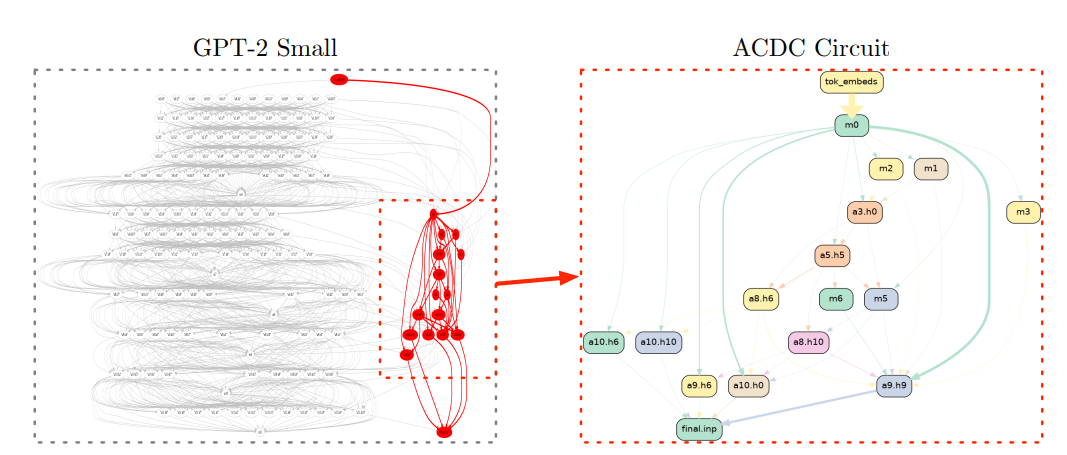
\includegraphics[width=0.9\textwidth]{gpt.png}
		
		\vspace{0.4em}
		{\footnotesize
			Automatically discovering circuits with ACDC.
			Left: Computational graph for GPT-2 Small with the recovered IOI circuit
			highlighted in red (edges shown only between adjacent layers).
			Right: Recovered circuit with labeled nodes; all identified heads belong
			to the IOI circuit. Edge thickness denotes relative importance.
		}
	\end{frame}
	
	%------------------------------------------------
	% 3 - A Common Interpretability Workflow
	%------------------------------------------------
	\begin{frame}{A Common Interpretability Workflow}
		\begin{itemize}
			\setstretch{1.5}
			\item \justifying Prior mechanistic interpretability studies implicitly
			follow a similar procedure for circuit discovery.
			
			\item \justifying This work makes that procedure \textbf{explicit}
			by identifying a common workflow across studies.
			
			\item \justifying The workflow decomposes circuit discovery into
			\textbf{well-defined stages}, separating:
			\begin{itemize}
				\item task and metric selection
				\item model representation
				\item circuit extraction
			\end{itemize}
			
			\item \justifying Formalizing this workflow clarifies
			where interpretability effort is currently concentrated.
		\end{itemize}
	\end{frame}
	
	%------------------------------------------------
	% 4 - Mechanistic Interpretability Workflow
	%------------------------------------------------
	\begin{frame}{Mechanistic Interpretability Workflow}
		\begin{itemize}
			\setstretch{1.4}
			\item \justifying Mechanistic interpretability studies across the literature
			follow a common \textbf{three-step workflow}.
			
			\item \justifying \textbf{Step 1:} Select a specific behavior and define
			an appropriate dataset and evaluation metric.
			
			\item \justifying \textbf{Step 2:} Represent the model as a
			\textbf{computational graph} at a chosen level of abstraction.
			
			\item \justifying \textbf{Step 3:} Identify a \textbf{circuit} by iteratively
			pruning components using activation patching.
			
			\item \justifying After circuit extraction, researchers interpret the
			functional roles of the remaining components.
		\end{itemize}
	\end{frame}
	
	%------------------------------------------------
	% 5 - Mechanistic Interpretability Workflow Diagram
	%------------------------------------------------
	\begin{frame}{Mechanistic Interpretability Workflow}
		\centering
		\includegraphics[width=0.9\textwidth]{fig2.png}
		
		\vspace{16pt}
		\scriptsize
		A common three-step workflow for circuit discovery observed across
		mechanistic interpretability studies, highlighting the circuit
		extraction stage addressed in this work.
	\end{frame}
	
	%------------------------------------------------
	% 6 - Step 1: Behavior, Dataset, and Metric
	%------------------------------------------------
	\begin{frame}{Step 1: Behavior, Dataset, and Metric}
		\begin{itemize}
			\setstretch{1.4}
			\item \justifying Mechanistic interpretability begins by selecting a
			\textbf{specific model behavior} to analyze.
			
			\item \justifying A dataset is constructed to reliably
			\textbf{elicit this behavior} from the trained model.
			
			\item \justifying Alongside the main dataset, a
			\textbf{corrupted dataset} is defined to disrupt the behavior
			while preserving surface structure.
			
			\item \justifying A quantitative \textbf{metric} is used to measure
			behavioral strength and compare patched or pruned models.
		\end{itemize}
	\end{frame}
	
	%------------------------------------------------
	% 7 - Example: Greater-Than Task
	%------------------------------------------------
	\begin{frame}{Example: Greater-Than Task}
		\begin{itemize}
			\setstretch{1.4}
			\item \justifying The \textbf{Greater-Than} task studies numerical
			comparison behavior in language models.
			
			\item Example prompt:
			\begin{itemize}
				\item ``The war lasted from 1517 to 15''
			\end{itemize}
			
			\item \justifying The model assigns higher probability to
			completions greater than \textbf{17}.
			
			\item \justifying This task provides a clear, well-defined behavior
			for circuit discovery experiments.
		\end{itemize}
	\end{frame}
	
	\begin{frame}{Automatically Discovered Circuits with ACDC}
		\centering
		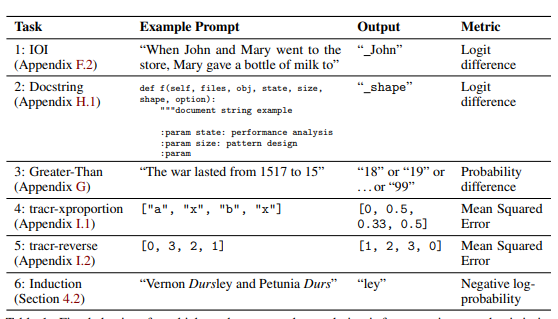
\includegraphics[width=0.9\textwidth]{table.png}
		
		\vspace{0.4em}
		{\scriptsize
			Five behaviors for which we have an end-to-end circuit from previous mechanistic interpretability work, plus Induction. We automatically rediscover the circuits for behaviors 1-5 in
			Section 4. Tokens beginning with space have a “ ” prepended for clarity.
		}
	\end{frame}

	
	%------------------------------------------------
	% 9 - Step 2: Computational Graph Representation
	%------------------------------------------------
	\begin{frame}{Step 2: Computational Graph Representation}
		\begin{itemize}
			\setstretch{1.7}
			\item \justifying To identify circuits, the model is represented as a
			\textbf{directed acyclic computational graph}.
			
			\item \justifying Nodes correspond to model components, and
			edges represent the \textbf{flow of information}.
			
			\item \justifying The choice of graph abstraction determines the
			\textbf{granularity} of the resulting circuit.
			
			\item \justifying This representation defines the search space
			for circuit extraction.
		\end{itemize}
	\end{frame}
	
	%------------------------------------------------
	% 10 - Step 2: Levels of Abstraction
	%------------------------------------------------
	\begin{frame}{Step 2: Levels of Abstraction}
		\begin{itemize}
			\setstretch{1.7}
			\item Computational graphs can be defined at
			different levels of abstraction.
			
			\item Examples include:
			\begin{itemize}
				\item attention heads and MLP layers
				\item query, key, and value paths
				\item individual neurons
				\item token-position-specific nodes
			\end{itemize}
			
			\item \justifying Finer abstractions yield more detailed circuits
			but increase computational cost.
		\end{itemize}
	\end{frame}
	
	%------------------------------------------------
	% 11 - Computational Graph Illustration
	%------------------------------------------------
	\begin{frame}{Computational Graph Illustration}
		\centering
		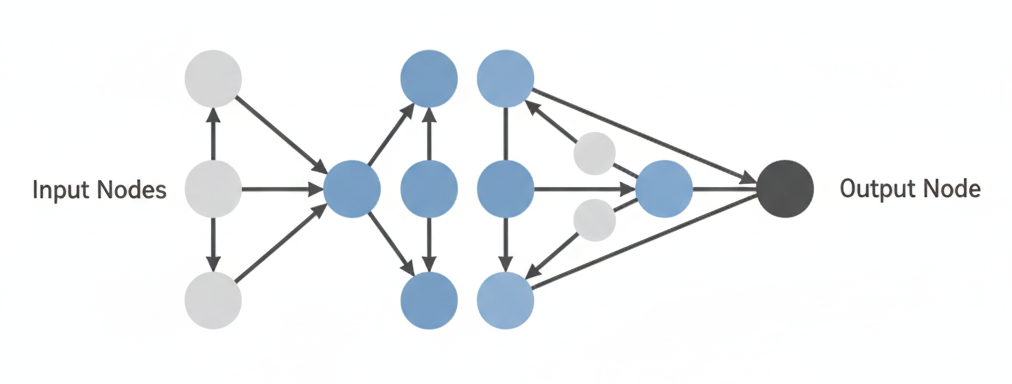
\includegraphics[width=0.9\textwidth]{fig5.png}
		
		\vspace{14pt}
		\scriptsize
		Schematic representation of a directed acyclic computational graph,
		where nodes denote model components and edges represent information
		flow toward the output.
	\end{frame}
	
	%------------------------------------------------
	% 12 - Step 3: Activation Patching
	%------------------------------------------------
	\begin{frame}{Step 3: Activation Patching}
		\begin{itemize}
			\setstretch{1.4}
			\item \justifying Circuit extraction proceeds by
			\textbf{activation patching} on the computational graph.
			
			\item \justifying Activations of nodes or edges are replaced with
			values from a \textbf{corrupted dataset}.
			
			\item \justifying The model is evaluated using the
			predefined metric to measure behavioral change.
			
			\item \justifying Components whose removal significantly degrades
			performance are considered important for the behavior.
		\end{itemize}
	\end{frame}
	
	%------------------------------------------------
	% 13 - Step 3: Recursive Circuit Extraction
	%------------------------------------------------
	\begin{frame}{Step 3: Recursive Circuit Extraction}
		\begin{itemize}
			\setstretch{1.7}
			\item \justifying Circuit discovery begins at the
			\textbf{output node} of the computational graph.
			
			\item \justifying Incoming edges are tested individually
			using activation patching.
			
			\item \justifying Edges with negligible impact on the metric
			are pruned from the graph.
			
			\item \justifying This process is applied \textbf{recursively},
			traversing backward through the graph.
		\end{itemize}
	\end{frame}
	
	%------------------------------------------------
	% 14 - Activation Patching Mechanism
	%------------------------------------------------
	\begin{frame}{Activation Patching Mechanism}
		\centering
		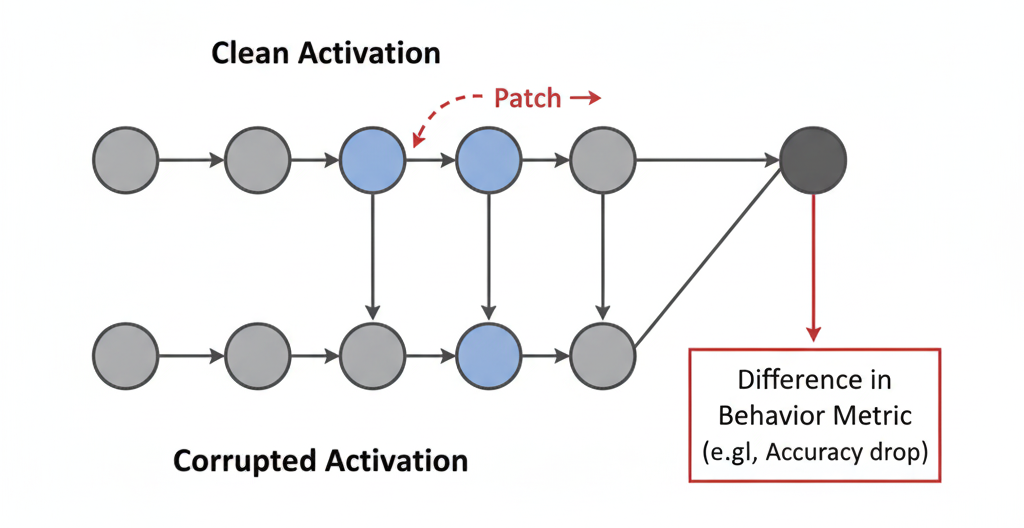
\includegraphics[width=0.9\textwidth]{fig6.png}
		
		\vspace{14pt}
		\scriptsize
		Activation patching compares model behavior under clean and corrupted
		activations by replacing internal values and measuring changes in
		the task-specific behavior metric.
	\end{frame}
	
	%------------------------------------------------
	% 15 - Automatic Circuit DisCovery (ACDC)
	%------------------------------------------------
	\begin{frame}{Automatic Circuit DisCovery (ACDC)}
		\begin{itemize}
			\setstretch{1.4}
			\item \justifying \textbf{Automatic Circuit DisCovery (ACDC)} is proposed
			to automate circuit extraction in mechanistic interpretability.
			
			\item \justifying Prior work relied on \textbf{manual, iterative}
			activation patching guided by human intuition.
			
			\item \justifying ACDC systematizes this process by
			automatically testing and pruning connections in
			the computational graph.
			
			\item \justifying The method outputs a \textbf{sparse circuit}
			that preserves performance on a chosen behavior.
		\end{itemize}
	\end{frame}
	
	
	%------------------------------------------------
	% 16 - Circuit Discovery through Pruning
	%------------------------------------------------
	\begin{frame}{Circuit Discovery through Pruning}
		\centering
		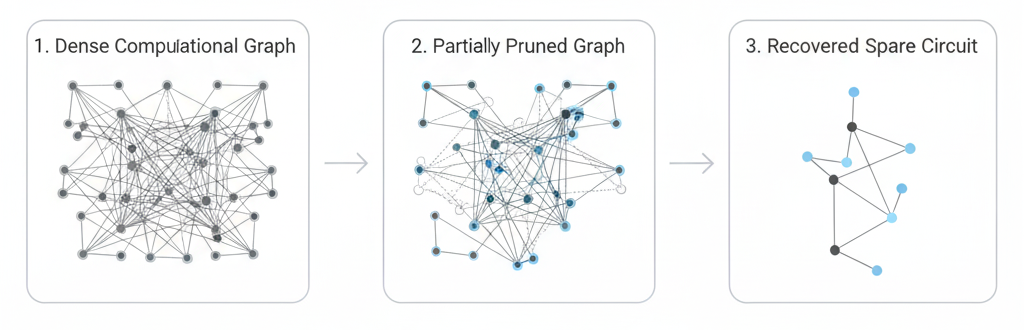
\includegraphics[width=0.9\textwidth]{fig7.png}
		
		\vspace{14pt}
		\scriptsize
		Progressive pruning of a dense computational graph into a sparse
		circuit, illustrating the objective of circuit discovery methods
		such as ACDC.
	\end{frame}
	
	%------------------------------------------------
	% 17 - ACDC: Algorithmic Overview
	%------------------------------------------------
	\begin{frame}{ACDC: Algorithmic Overview}
		\begin{itemize}
			\setstretch{1.4}
			\item \justifying ACDC operates on a fixed computational graph
			and a predefined behavior metric.
			
			\item \justifying Starting from the \textbf{output node}, incoming
			edges are evaluated using activation patching.
			
			\item \justifying An edge is removed if replacing its activation
			with corrupted values does not significantly
			change the metric.
			
			\item \justifying The procedure proceeds \textbf{recursively in
				reverse topological order} until a minimal circuit
			is recovered.
		\end{itemize}
	\end{frame}
	
	%------------------------------------------------
	% ACDC Algorithm (Formal Reference)
	%------------------------------------------------
	\begin{frame}{ACDC Algorithm (Formal Reference)}
		\centering
		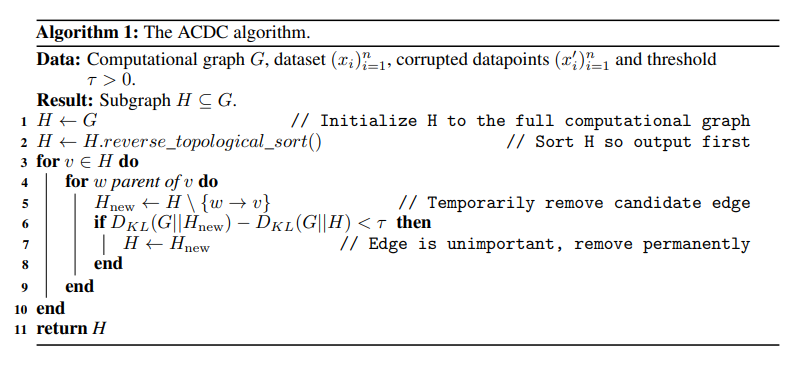
\includegraphics[width=0.9\textwidth]{fig8.png}
		
		\vspace{10pt}
		\scriptsize
		Formal description of the Automatic Circuit DisCovery (ACDC)
		algorithm.
	\end{frame}
	
	%------------------------------------------------
	% 8 - ACDC Greater-Than Circuit Diagram
	%------------------------------------------------
	\begin{frame}{Automatic Circuit Discovery: Greater-Than Task}
		\centering
		\vspace{5pt}
		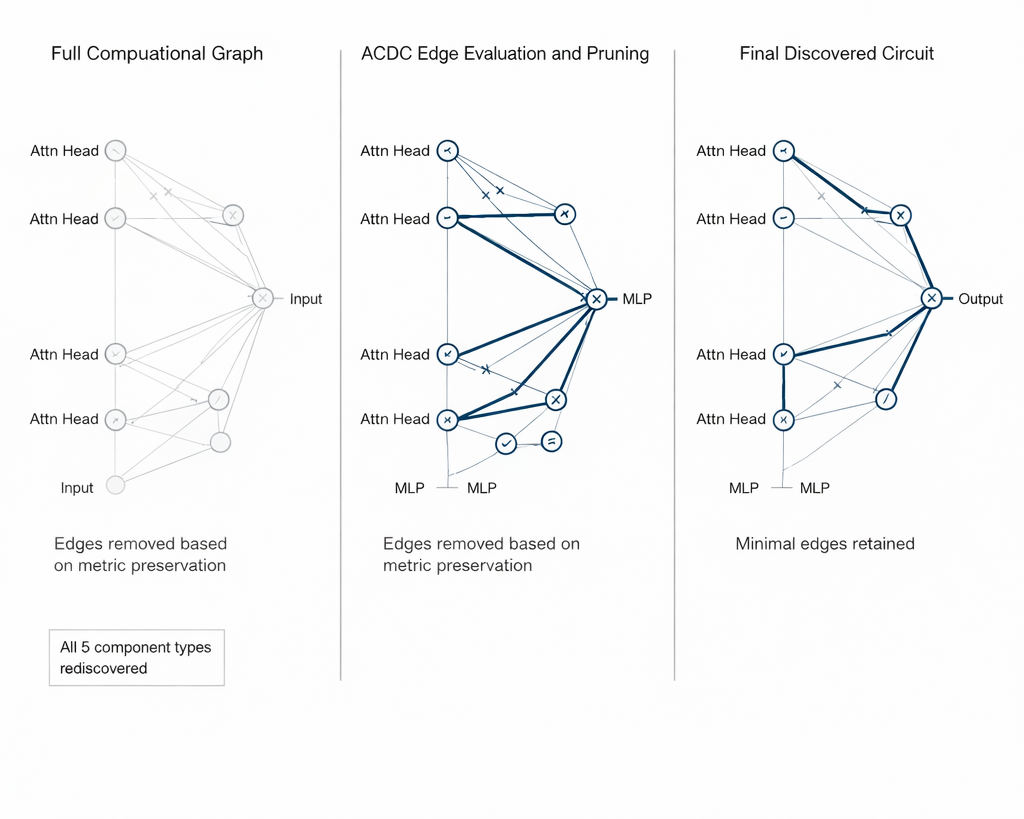
\includegraphics[width=0.85\textwidth]{fig1.png}
		
		%	\vspace{2pt}
		\scriptsize
		Circuit recovered by Automatic Circuit Discovery (ACDC) for the
		Greater-Than task in GPT-2 Small. The method prunes the full
		computational graph to a sparse subgraph that preserves task
		performance.
	\end{frame}
	
	%------------------------------------------------
	% 20 - Evaluation Objectives
	%------------------------------------------------
	\begin{frame}{Evaluation Objectives}
		\begin{itemize}
			\setstretch{1.5}
			\item \justifying The evaluation focuses on assessing the
			\textbf{quality of circuits} recovered by ACDC.
			
			\item Two primary questions are investigated:
			\begin{itemize}
				\item \textbf{Q1:} Does ACDC recover circuits that
				preserve task performance?
				
				\item \textbf{Q2:} How do recovered circuits compare
				to those obtained by prior methods?
			\end{itemize}
			
			\item \justifying Evaluation is performed across multiple tasks
			and levels of abstraction.
		\end{itemize}
	\end{frame}
	
	%------------------------------------------------
	% 21 - Baselines for Circuit Discovery
	%------------------------------------------------
	\begin{frame}{Baselines for Circuit Discovery}
		\begin{itemize}
			\setstretch{1.6}
			\item \justifying ACDC is compared against prior circuit discovery
			and pruning approaches.
			
			\item \textbf{Subnetwork Probing (SP):}
			\begin{itemize}
				\item Identifies subnetworks by optimizing masks
				over model components.
			\end{itemize}
			
			\item \textbf{Head Importance Score for Pruning (HISP):}
			\begin{itemize}
				\item Prunes attention heads based on importance scores.
			\end{itemize}
			
			\item These methods serve as reference points
			for circuit recovery quality.
		\end{itemize}
	\end{frame}
	
	\begin{frame}{Evaluation: Performance–Sparsity Trade-off}
		\centering
		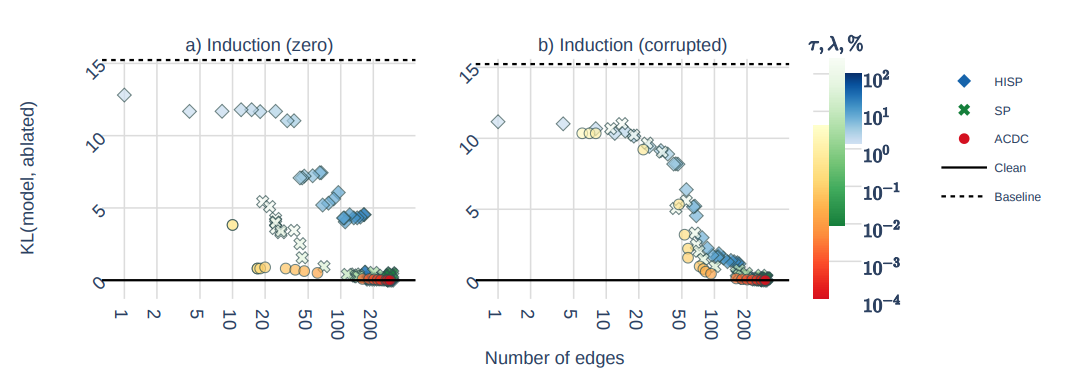
\includegraphics[width=0.95\textwidth]{fig9.png}
		
		
		\vspace{8pt}
		\scriptsize
		KL divergence versus number of edges for circuits recovered on the
		Induction task. ACDC (red) achieves lower divergence with fewer edges
		compared to SP and HISP, under both zero and corrupted activation patching.
	\end{frame}
	
	\begin{frame}{Evaluation: Recovery vs.\ Prior Circuits}
		\begin{itemize}
			\item Circuit discovery is evaluated by comparison with
			canonical circuits reported in prior mechanistic
			interpretability studies.
			
			\item Circuit recovery is formulated as a
			\textbf{binary classification problem} over edges:
			\begin{itemize}
				\item edge belongs to the circuit
				\item edge does not belong to the circuit
			\end{itemize}
			
			\item Performance is summarized using
			\textbf{ROC curves} and the
			\textbf{Area Under the Curve (AUC)}.
			
			\item High true-positive rates indicate recovery of known
			circuit components (Q1), while low false-positive rates
			reflect exclusion of irrelevant components (Q2).
		\end{itemize}
	\end{frame}
	
	\begin{frame}{Evaluation: Stand-alone Circuit Properties}
		\begin{itemize}
			\item To avoid reliance on imperfect human-annotated circuits,
			the authors also evaluate intrinsic properties of the
			recovered subgraphs.
			
			\item Circuit quality is assessed using:
			\begin{itemize}
				\item similarity of circuit behavior to the original model
				\item number of edges retained in the circuit
			\end{itemize}
			
			\item A high-quality circuit preserves the target behavior
			while remaining sparse.
			
			\item This evaluation provides indirect evidence for both
			recovery quality (Q1) and exclusion of irrelevant components
			(Q2).
		\end{itemize}
	\end{frame}
	
	%------------------------------------------------
	% 22 - High-Level Evaluation Findings
	%------------------------------------------------
	\begin{frame}{High-Level Evaluation Findings}
		\begin{itemize}
			\setstretch{1.6}
			\item \justifying ACDC successfully recovers sparse circuits
			that preserve task performance across evaluated tasks.
			
			\item \justifying In several settings, ACDC identifies
			\textbf{smaller or comparable circuits} relative
			to baseline methods.
			
			\item Circuit quality is sensitive to:
			\begin{itemize}
				\item choice of behavior metric
				\item corrupted dataset construction
				\item graph abstraction level
			\end{itemize}
		\end{itemize}
	\end{frame}
	
	%------------------------------------------------
	% 23 - Limitations and Scope
	%------------------------------------------------
	\begin{frame}{Limitations and Scope}
		\begin{itemize}
			\setstretch{1.7}
			\item ACDC does not automate the
			\textbf{interpretation} of recovered circuits.
			
			\item Results depend on:
			\begin{itemize}
				\item the selected behavior and dataset
				\item the abstraction of the computational graph
			\end{itemize}
			
			\item Circuit discovery is performed
			\textbf{post-hoc} on trained models.
			
			\item \justifying The method does not provide guarantees
			of uniqueness or causal correctness.
		\end{itemize}
	\end{frame}
	
	%------------------------------------------------
	% 24 - Conclusion
	%------------------------------------------------
	\begin{frame}{Conclusion}
		\begin{itemize}
			\justifying
			\setstretch{1.8}
			\item This work systematizes a common workflow
			for mechanistic interpretability.
			
			\item ACDC automates circuit extraction using
			activation patching and recursive pruning.
			
			\item The approach scales circuit discovery
			beyond manual analysis.
			
			\item Automating circuit interpretation
			remains an open research direction.
		\end{itemize}
	\end{frame}
	
	%------------------------------------------------
	% 25 - Mathematical Foundations (Appendix)
	%------------------------------------------------
	\begin{frame}{Mathematical Foundations (Appendix)}
		\begin{itemize}
			\setstretch{1.15}
			
			\item \justifying
			The appendix formalizes the mathematical foundations that
			underpin the Automatic Circuit Discovery (ACDC) framework.
			
			\item \justifying
			Circuit quality is quantified using the
			\textbf{Kullback--Leibler (KL) divergence} between the output
			distribution of the original model and that of the pruned
			subgraph.
			
			\item \justifying
			Edge pruning is governed by a
			\textbf{threshold-based criterion}, where edges are removed
			if their contribution induces only a negligible change in
			the evaluation metric.
			
			\item \justifying
			Additional analyses include:
			\begin{itemize}
				\item \justifying alternative evaluation metrics (e.g., logit difference)
				\item \justifying comparison between zero and corrupted activation patching
				\item \justifying robustness checks and identified failure cases
			\end{itemize}
			
			\item \justifying
			These results collectively support both the correctness
			and the documented limitations of the proposed method.
		\end{itemize}
	\end{frame}
	
	
	\begin{frame}{Backup: ACDC Pruning Criterion}
		\small
		
		An edge $(w \rightarrow v)$ is removed if:
		\[
		\mathrm{DKL}(G \parallel H_{\text{new}}) - 
		\mathrm{DKL}(G \parallel H) < \tau
		\]
		where:
		\begin{itemize}
			\item $G$ is the full model
			\item $H$ is the current subgraph
			\item $\tau$ is a sparsity threshold
		\end{itemize}
	\end{frame}
	
	%------------------------------------------------%------------------------------------------------%------------------------------------------------%------------------------------------------------%------------------------------------------------%------------------------------------------------%------------------------------------------------%------------------------------------------------%------------------------------------------------%------------------------------------------------%------------------------------------------------%------------------------------------------------%------------------------------------------------%------------------------------------------------%------------------------------------------------%------------------------------------------------%------------------------------------------------%------------------------------------------------%------------------------------------------------	
	
	
	%------------------------------------------------
	% ACDC Procedure Summary
	%------------------------------------------------
	\begin{frame}{How ACDC Works (Summary)}
		\begin{itemize}
			\setstretch{1.4}
			\item Step a: specify task, computational graph, and threshold $\tau$.
			\item Step b: evaluate each connection by activation patching.
			\item Step c: prune connections with metric impact below $\tau$.
			\item Recursively apply until the full circuit is recovered.
		\end{itemize}
		
		\vspace{4pt}
		\scriptsize
		\centering
		ACDC returns a minimal subgraph that preserves task performance.
	\end{frame}
	
	%------------------------------------------------
	% Thank You Slide
	%------------------------------------------------
	\begin{frame}
		\centering
		\Large Thank You
	\end{frame}
	
\end{document}